\subsubsection{12.12.2015}
\textit{\textbf{Time frame:}} 16:00-22:00 

The opposite pairs of slats on the elevator were connected by the ribs. It strengthened the elevator and made it more stable as from now on both sides will move dependently (figure \ref{Elevator2.3}, \ref{Elevator2.4}).

\begin{figure}[H]
	\begin{minipage}[h]{0.47\linewidth}
		\center{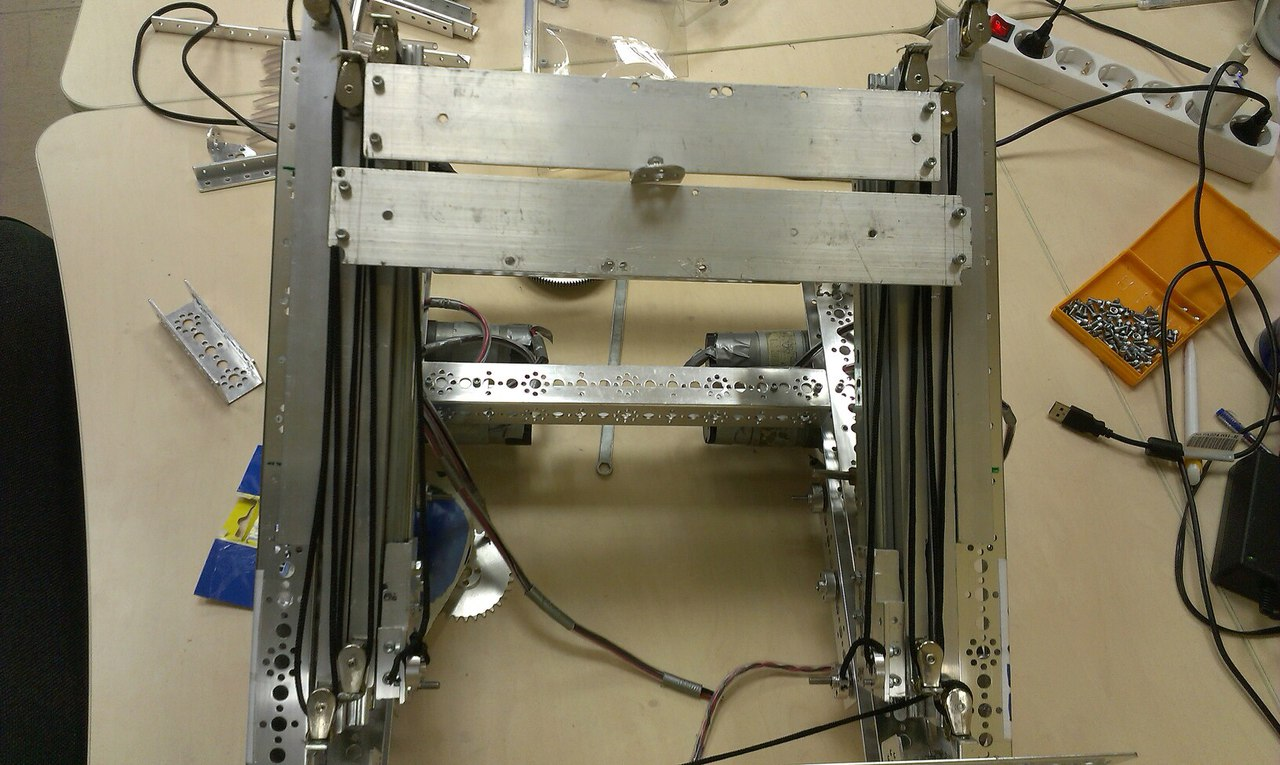
\includegraphics[scale=0.2]{3Engineering/5Team_meetings/days_of_meetings/2015.12.12/images/01}}
		\caption{Slats connected by the ribs 1}
		\label{Elevator2.3}
	\end{minipage}
	\hfill
	\begin{minipage}[h]{0.47\linewidth}
		\center{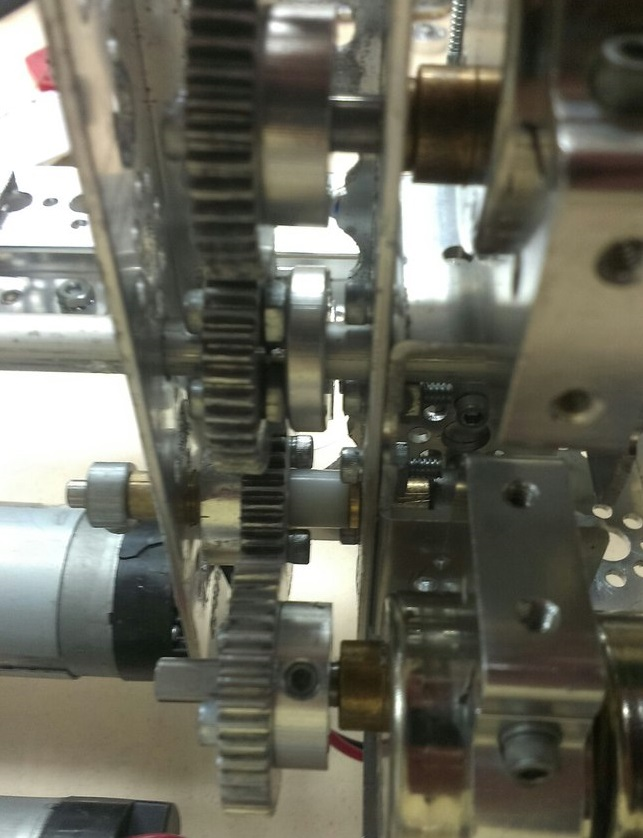
\includegraphics[scale=0.2]{3Engineering/5Team_meetings/days_of_meetings/2015.12.12/images/02}}
		\caption{Slats connected by the ribs 2}
		\label{Elevator2.4}
	\end{minipage}
\end{figure}

In addition, it was started the assembling of the winch for extracting lift. It will include two distinct reels for two ropes from both sides of the lift (figure \ref{Winch2.1}). 

At first, it was an idea to make each coil from two middle-sized gears with screws between them, but this construction was too bulky. So, it was decided to apply wheels from TETRIX caterpillar tracks as coils.

\begin{figure}[H]
	\begin{minipage}[h]{1\linewidth}
		\center{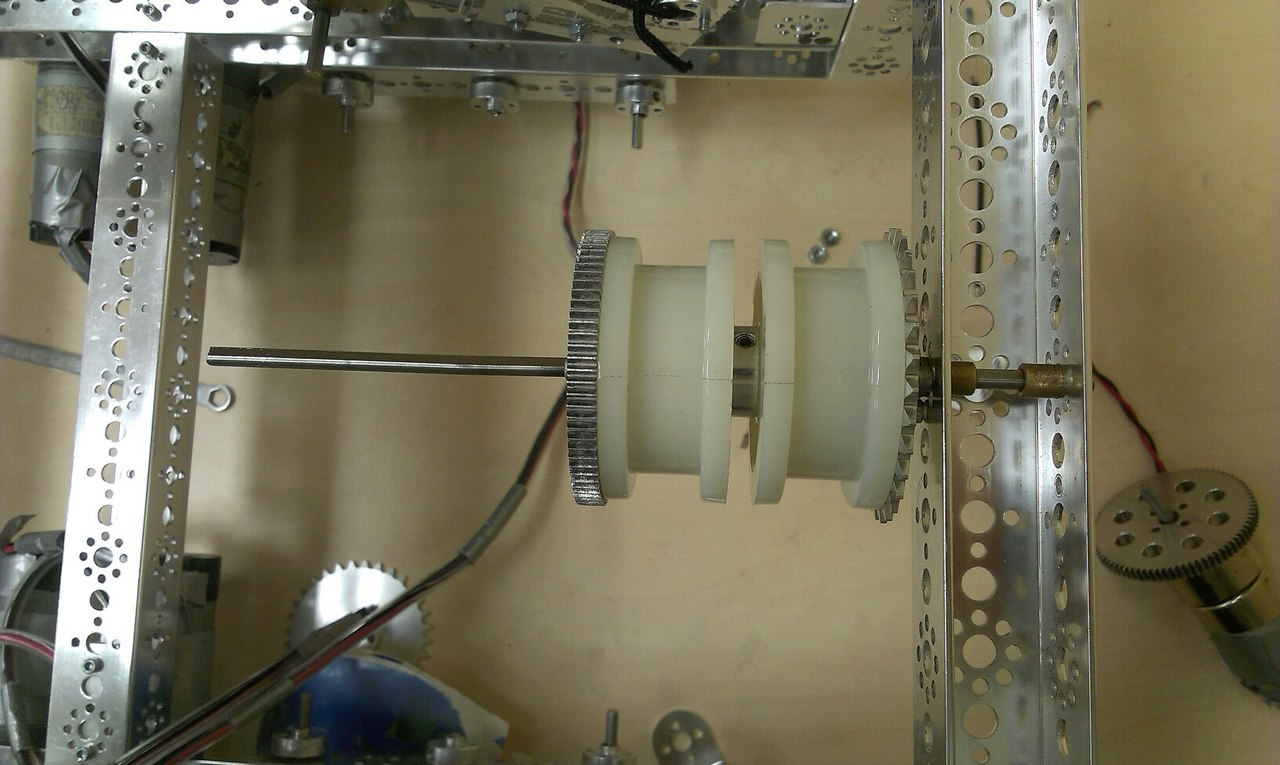
\includegraphics[scale=0.2]{3Engineering/5Team_meetings/days_of_meetings/2015.12.12/images/03}}
		\caption{Winch was created}
		\label{Winch2.1}
	\end{minipage}
\end{figure}
